\chapter{Bayesian Fusion Convergence (Study 12)}
\label{appendix:bayesian-fusion-charts}

Step-by-step parameter commentary for the claims-only scenario in Study~12 (Section~\ref{subsec:study-12-bayesian-conflict-resolution}; Tables~\ref{tab:bayesian-scenario-comparison} and~\ref{tab:bayesian-walkthrough}).

\subsection*{Step-by-Step Walkthrough}
\label{appendix:bayesian-fusion-walkthrough}

\subsubsection{Step 1: CV assertion.}
We start from a sparse prior ($\alpha_0 = \beta_0 = 0.1$, score $0.500$), with repeated CV 
mentions leading to a strong signal ($s_1 = 0.8$, $c_1 = 0.5$), lifting the score to $0.711$ ($\alpha = 0.505$, $\beta = 0.205$, 
$\sigma$: $0.456 \rightarrow 0.347$). On CV text alone, the candidate looks like a strong match, and this would usually be 
the outcome of a CV-only screening pipeline.

\subsubsection{Step 2: GitHub contradiction.}
Zero GitHub signal ($s_2 = 0.0$, $c_2 = 0.9$) pulls the score to $0.314$ 
($\beta = 1.106$). A confident verifiable contradiction overrides the CV claim. Proprietary work without public 
repos records uncertainty rather than a hard rejection. Alternatively, could be a candidate who has demonstrated evidence
for other skills, but not the one in question.

\subsubsection{Step 3: LinkedIn endorsement.}
Claimed LinkedIn ($s_3 = 0.8$, $c_3 = 0.2$) nudges the score to $0.369$ 
only. Self-report cannot replace demonstrated evidence. Given frequent CV embellishment, MERIT intentionally 
favours candidates who can show public work.

\textbf{Demonstration-only profile.} For the demonstration-only profile ($s_1 = 0.0, s_2 = 1.0, s_3 = 0.0$), an initial lack of CV mentions causes the score to dip to $0.148$. However, a perfect GitHub validation ($s_{\mathrm{GH}} = 1.0$) aggressively pulls the score up to $0.624$, settling at $0.555$ after LinkedIn. Despite having more overall text dedicated to it, the claims-only profile finishes 19 points lower ($0.369$). See Table~\ref{tab:bayesian-scenario-comparison} and the right column of Figure~\ref{fig:bayesian-fusion-convergence} for a final visual comparison of these bounds.

\begin{figure}[htbp]
    \centering
    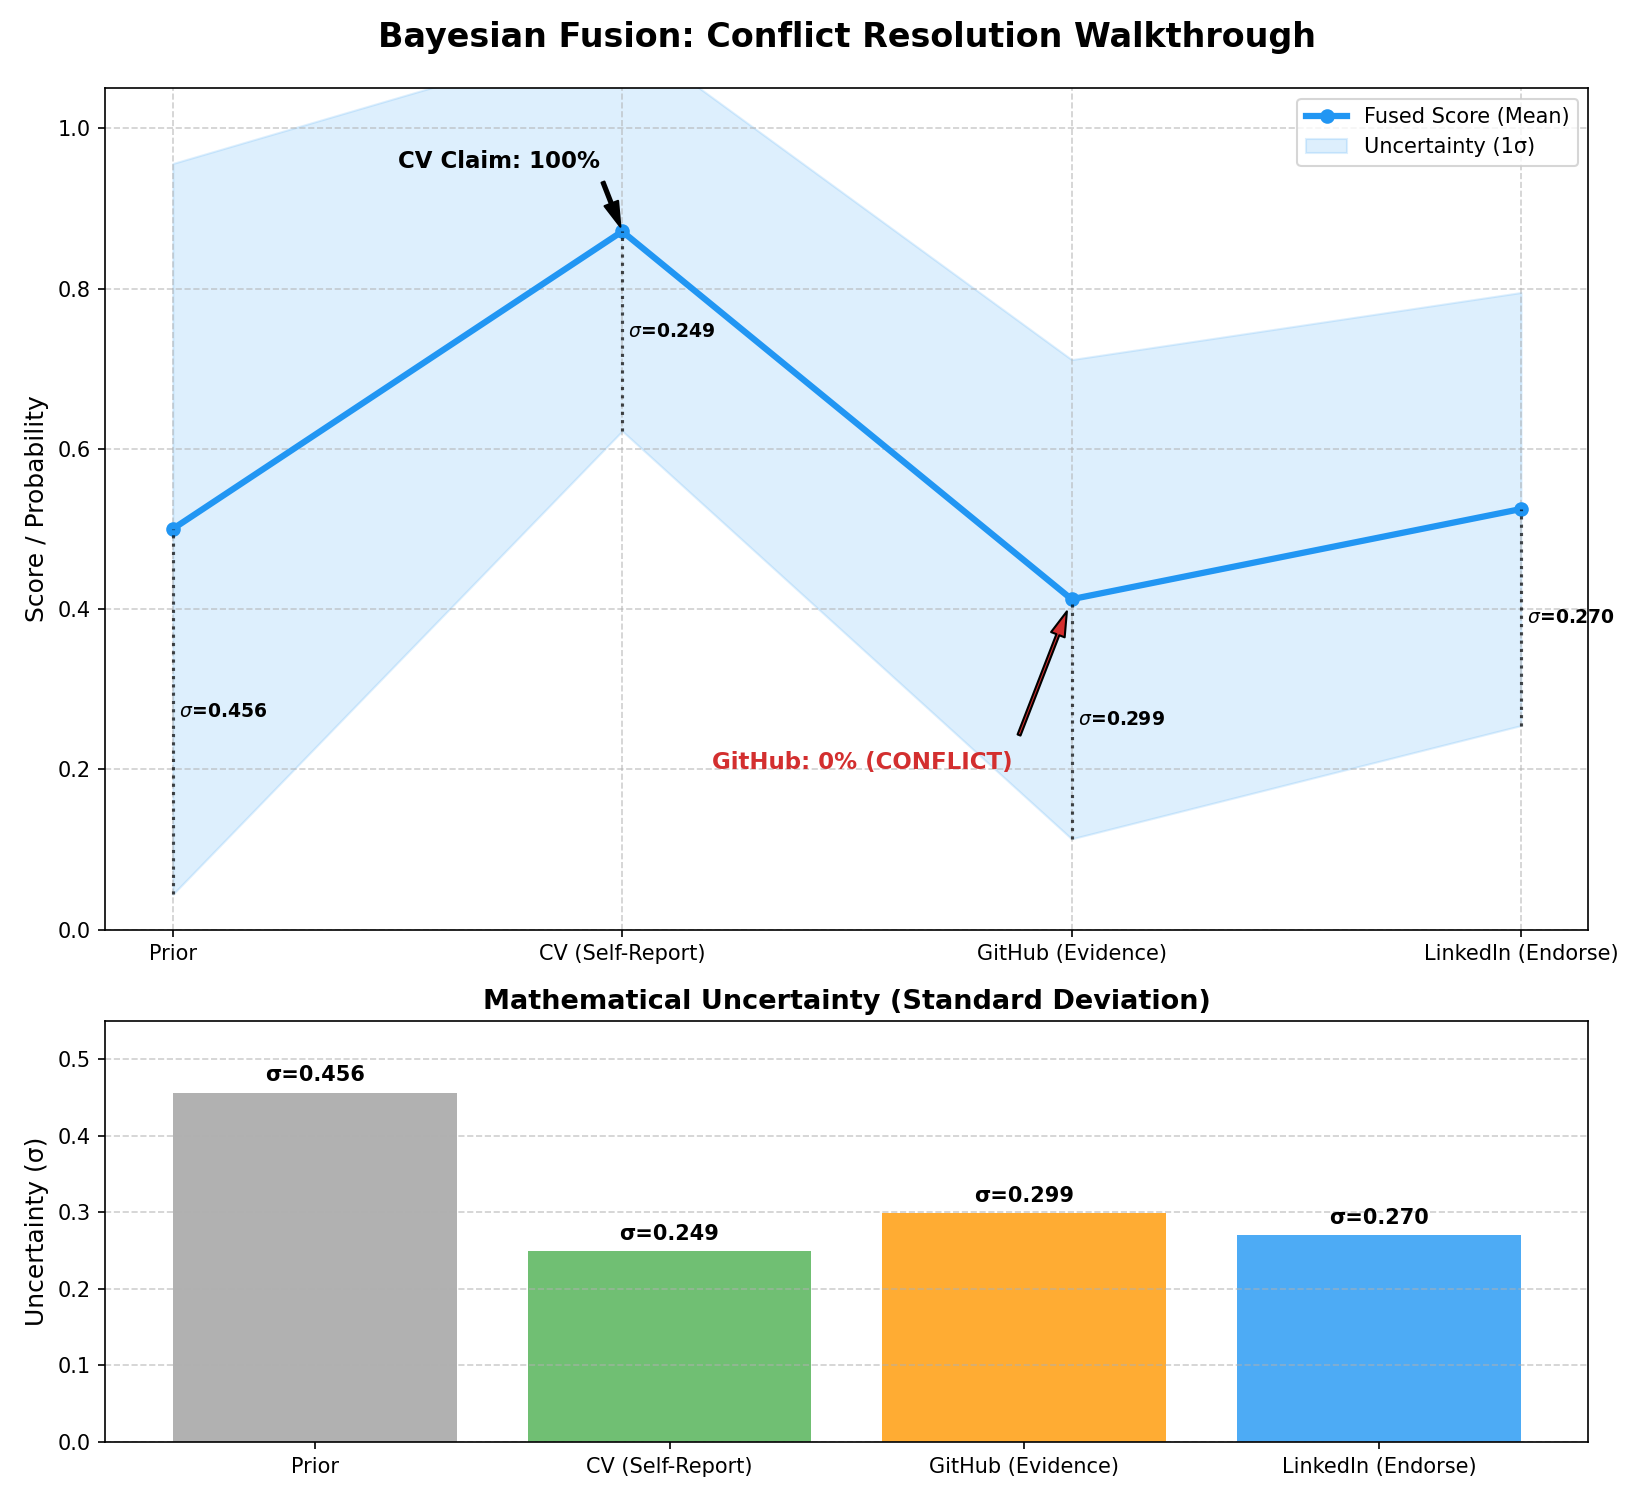
\includegraphics[width=\textwidth,height=0.30\textheight,keepaspectratio]{../evaluation/12-conflict_resolution/output/fusion_convergence_detailed.png}
    \caption[Study~12: Fusion convergence]{Study~12: Beta fusion for claims-only (left) vs.\ demonstration-only (right) profiles; top panels = fused score, bottom panels = $\sigma$ by step.}
    \label{fig:bayesian-fusion-convergence}
\end{figure}

\clearpage
\subsection*{Empirical Bounds}
For completeness, Figure~\ref{fig:bayesian-fusion-convergence-bounds} presents the trajectories for the empirical bounds: the full-evidence scenario (where all sources provide maximum possible validation) and the zero-evidence scenario (where all evaluated sources return zero signal). The full-evidence profile quickly converges to the $0.861$ ceiling, while the zero-evidence profile collapses to the $0.062$ floor.

\textbf{Full-evidence profile.} Here, the CV assertion provides a strong initial signal ($s_1=0.8, c_1=0.5$), raising the expected score. A subsequent perfect GitHub validation ($s_2=1.0, c_2=0.9$) aggressively drives the score upwards while dramatically collapsing the uncertainty ($\sigma = 0.207$). A final LinkedIn endorsement ($s_3=0.8, c_3=0.2$) provides a minor additional boost, pushing the engine to its strict mathematical ceiling of $0.861$. The standard deviation of $0.206$ represents the absolute minimum uncertainty achievable with this three-source configuration.

\textbf{Zero-evidence profile.} Conversely, if all sources are systematically evaluated but found to be completely devoid of target skills ($s_1=0.0, s_2=0.0, s_3=0.0$), the engine progressively penalises the candidate. By the time GitHub returns a null signal with high confidence ($c_2=0.9$), the score drops sharply, ultimately bottoming out at the mathematical floor of $0.062$. This confirms that candidates with zero demonstrated skills cannot coast on the prior, preventing them from unfairly outranking candidates with weak but non-zero evidence.

\begin{figure}[H]
    \centering
    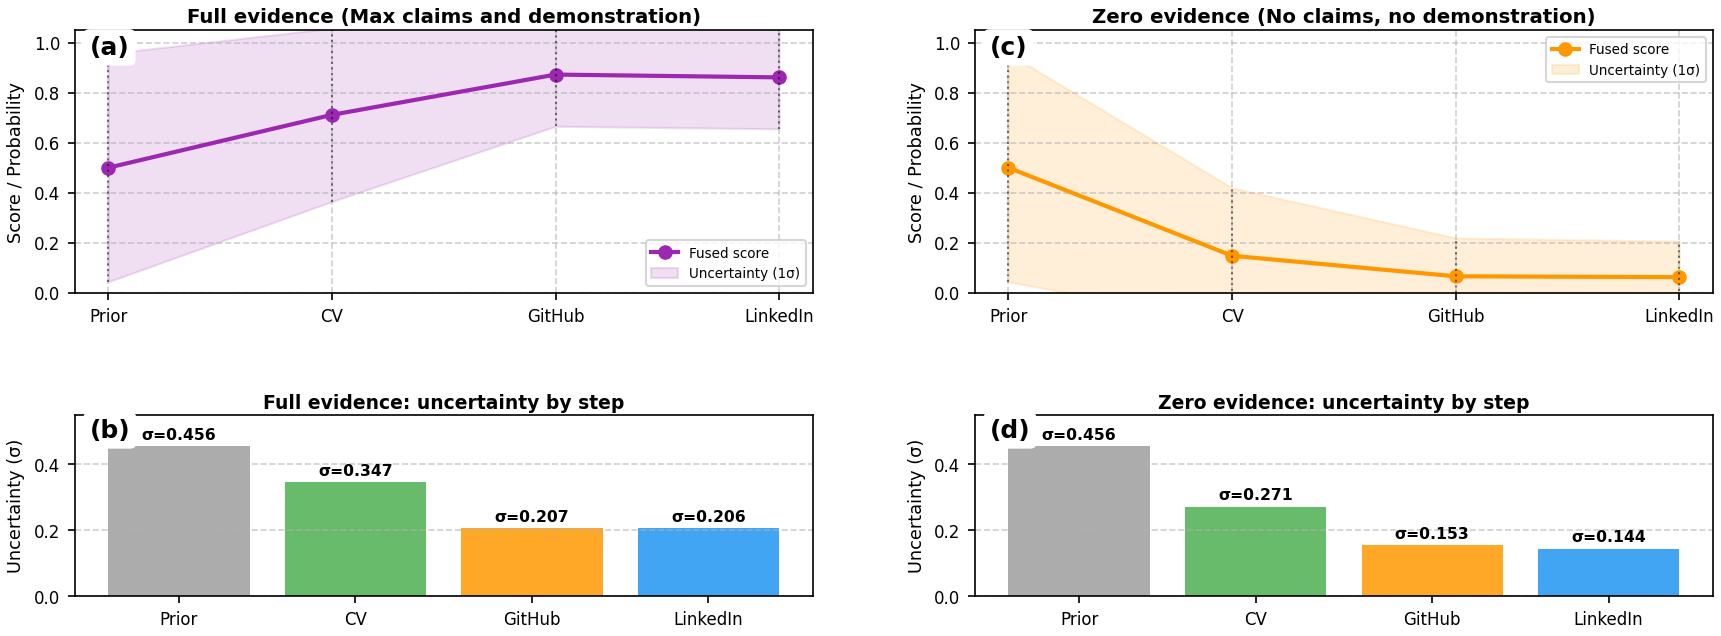
\includegraphics[width=\textwidth,height=0.30\textheight,keepaspectratio]{../evaluation/12-conflict_resolution/output/fusion_convergence_bounds.png}
    \caption[Study~12: Fusion convergence bounds]{Study~12: Beta fusion for the theoretical upper bound (full evidence, left) vs.\ lower bound (zero evidence, right); top panels = fused score, bottom panels = $\sigma$ by step.}
    \label{fig:bayesian-fusion-convergence-bounds}
\end{figure}
